\documentclass[fontsize=12bp, paper=a4]{scrarticle}
\usepackage[utf8]{inputenc}

\usepackage[english,main=serbian]{babel}
\usepackage[left=2cm, right=2cm, top=3cm, bottom=3cm]{geometry}
\usepackage[automark]{scrlayer-scrpage}
\usepackage{ragged2e}
\usepackage{amsmath}
\usepackage{mathabx}
\usepackage{hyperref}
\usepackage{graphicx}
\usepackage{wrapfig}
\usepackage{amssymb}
\usepackage{listings}
\usepackage{xcolor}
\usepackage{xurl}
\usepackage{csquotes}
%\usepackage[backend=biber, style=numeric]{biblatex}

%
\definecolor{codegreen}{rgb}{0,0.6,0}
\definecolor{codegray}{rgb}{0.5,0.5,0.5}
\definecolor{codepurple}{rgb}{0.58,0,0.82}
\definecolor{backcolour}{rgb}{0.95,0.95,0.92}

\lstdefinestyle{mystyle}{
    backgroundcolor=\color{backcolour},   
    commentstyle=\color{codegreen},
    keywordstyle=\color{magenta},
    numberstyle=\tiny\color{codegray},
    stringstyle=\color{codepurple},
    basicstyle=\ttfamily\footnotesize,
    breakatwhitespace=false,         
    breaklines=true,                 
    captionpos=b,                    
    keepspaces=true,                 
    numbers=left,                    
    numbersep=5pt,                  
    showspaces=false,                
    showstringspaces=false,
    showtabs=false,                  
    tabsize=2
}

\lstset{style=mystyle}

\renewcommand\lstlistingname{Implementacija}
\renewcommand\lstlistlistingname{Implementacija}

%

\graphicspath{ {./images/} }

%
\title{Seminarski rad} 
\subtitle{iz predmeta Sistem za podršku odlučivanju}

\begin{document}

\begin{titlepage}
    \vspace{\stretch{1}}
    
    \begin{center}
        
        \vspace*{8cm}
        
        \large{Univerzitet u Kragujevcu}
        
        \vspace*{1cm}

        {\bfseries \LARGE Seminarski rad}
        
        \large{iz predmeta Sistem za podršku odlučivanju}
        
        \vspace*{1cm}
        \large{Tema:}

        \Large{Implementacija klasifikacija izveštaja o dijagnozama dijabetisa}


        \vspace*{2cm}
    \end{center}
    \hfill{\parbox[s]{8cm}{

    mentori: 
    \begin{tabular}{l}
        \\
        \\
        Ognjen Pavić, \\
        prof. dr. Tijana Geroski, \\
        prof. dr. Nenad Filipović 
    \end{tabular}
    
    student: \begin{tabular}{l}
        Željko Simić 3vi/2023
    \end{tabular}
    }}

    \hspace*{\fill} 

    \vspace*{2cm}

    \begin{center}
        Kragujevac 2024.
    \end{center}
\end{titlepage}


\setcounter{page}{1}
\justifying
\linespread{0.9}
\cfoot[\pagemark]{\pagemark}
\ofoot[]{}
\ohead[]{Željko Simić 3vi/2023}
\chead[]{}
\ihead[]{Univerzitet u Kragujevcu}
%
\justifying

\section{Uvod}
% Seminarski rad sastoji se iz dva dela:
% 1. Primena znanja iz algoritama masinskog ucenja za klasifikaciju koja podrazumeva analizu podataka u vidu 
%     - raspodele, 
%     - korelacije i
%     - neophodnih izmena skupa podataka i 
%     - kreiranje najtacnijeg klasifikacionog modela za resavanje konkretnog problema. 
    
% 2. Dokumentovanje
% celokupnog procesa izrade zadatka sto podrazumeva:
% - istrazivanje vezano za samu prirodu problema koji se resava
% - opis procesa analize podataka i moguce zakljucke do kojih ste dosli prilikom analize podataka
% - sve izmene seta podataka koje su doprinele dobijanju stabilnijeg i tacnijeg resenja prilikom kreiranja klasifikacionog modela kao i razlozi zbog
% kojih su te izmene smele biti napravljene
% - opis modela koji je proizveo najbolje rezultate
% - nacin na koji su rezultati interpretirani (koje metrike su koriscene za ocenjivanje razlicitih modela prilikom trazenja najboljeg)
% - opis postignutih rezultata najboljeg modela
% - izvedeni zakljucak o tome koji algoritam se pokazao najbolje i vase misljenje o tome zbog cega je taj algoritam postigao bolje rezultate u
% poredjenju sa ostalim isprobanim algoritmima

\subsection{Priroda problema}
Skup podataka koji se razmatra se tiče zapisnika napravljenih tokom posmatranja pacijenata koji se leče od bolesti dijabetesa u rasponu od nekoliko nedelja do nekoliko meseci zarad održavanja medicinskog simpozijuma 1994. u vezi ovog problema.\cite{diabetes} Automatizovani uređaj u sebi poseduje interni sat koji prati i zabeležava vreme određenih događaja. Papirni zapisnici imaju fiktivno uniformne ispraćena vremena unošenjem u zapisnik, gde elektronski uređaji imaju realistične vremenske zapise. 

Zapisnik o dijabetisu sadrže se od 4 polja po posebnom izveštaju.

\begin{enumerate}
    \itemsep0em
    \item \verb|Date| - datum u vidu formata \verb|MM-DD-YYYY|,
    \item \verb|Time| - vreme u \verb|XX:YY| formatu,
    \item \verb|Code| - šifrovano po slučaju stanja glukoze, insulina koje je ispraćeno ili svakodnevne aktivnosti koja je obavljena,
    \item \verb|Value| - vrednost koja ukazuje na količinu dijabetisa u krvi, tj. $\frac{mg}{dl}$.
\end{enumerate}

Svako posebno polje je izdeljeno tabulatorima i izveštaji u vidu zapisa izdeljeni po novoj liniji u više fajlova određenog za svakog pacijenata, služe da opišu fiziologiju i patofiziologiju šećerne bolesti i tretman.

\vbox{}

Šifre \verb|Code|-a imaju zasebno za sebe svoje značenje:
\begin{itemize}
    \itemsep0em
    \item  33 - regularna insulinska doza,
    \item 34 - NPH insulinska doza,
    \item 35 - UltraLente insulinska doza,
    \item 48 - Neodređena mera glukoze u krvi
    \item 57 - Neodređena mera glukoze u krvi
    \item 58 - Mera glukoze u krvi pre doručka
    \item 59 - Mera glukoze u krvi posle doručka
    \item 60 - Mera glukoze u krvi pre ručka
    \item  61 - Mera glukoze u krvi posle ručka
    \item 62 - Mera glukoze u krvi pre večere
    \item 63 - Mera glukoze u krvi posle večere
    \item 64 - Mera glukoze u krvi pre užine
    \item 65 - Hipoglikemički simptomi,
    \item 66 - Tipično uzimanje hrane,
    \item 67 - Uzimanje hrane više nego obično,
    \item 68 - Uzimanje hrane manje nego obično,
    \item 69 - Tipična fizička aktivnost,
    \item 70 - Fizička aktivnost više nego obično,
    \item 71 - Fizička aktivnost manje nego obično,
    \item 72 - Neodređen specijalan događaj.
\end{itemize}

\vbox{}

Vrednosti \verb|Value| imaju svoje neke raspone koje indiciraju određene ishode:
\begin{itemize}
    \itemsep0em
    \item Hipoglikemički simptom, manjak glukoze u krvi se javlja pri $<40 \frac{mg}{dl}$ i moguć uticaj nesvestice, dezorjentacije, letargije, slabosti, moždani udar;
    % regulation systems attempt to reverse the low BG.
    % the patient feels the effect off the adrenal hormone epinephrine as the BG
    \item Hipoglikemički simptom, $40 - 80 \frac{mg}{dl}$ - pacijent oseća efekat gašenja adrenalnog hormona epinefrina (glavobolje, stomačni bol, znoj) kako regulacioni sistemi glukoza u krvi preokreću manjak glukoze u krvi. Ako su simptomi neprijatni to ukazuje da glukoza u krvi opada do mere opasnosti;
    \item $80 - 120 \frac{mg}{dl}$ - normalan pred-obrokovno stanje glukoze u krvi,
    \item $80 - 140 \frac{mg}{dl}$ - normalno posle-obrokovno stanje,
    \item $<200\frac{mg}{dl}$ je stanje 90\% slučajeva, a prosečan slučaj je da imaju $150\frac{mg}{dl}$;
    \item $>200\frac{mg}{dl}$ dovodi do zdravstveno ugrožavajućih ishoda nakon dužeg vremena - vaskularne komplikacije.
\end{itemize}

Svaka insulinska formulacija ima svoj karakterističan vremenski opseg otkad počinje da deluje (O), vreme vrhunca aktivnosti (P), efektivnog trajanja (D). Na ove vremenske opsege mogu uveliko uticati većina faktora (mesto uboda - brzina apsorpcije delotvornija ubodom stomaka, umesto u glutealni mišić, da li je ljudski insulin ili životinjskog porekla).
\begin{itemize}
    \itemsep0em
    \item Regularni insulin - O 15-45 minuta - P 1-3 sata - D 4-6 sata,
    \item NPH insulin - O 1-3 sata - P 4-6 sata - D 10-14 sata,
    \item UltraLente - O 2-5 sata -  P nema isticajnih vrhunaca - D 24-30 sata.
\end{itemize}

I postoje i ostali uticaje na nivoe glukoze u krvi (ishrana, fizička aktivnost, itd.), ali na to nećemo da se osvrćemo nadalje.

\vbox{}

Pošto će se obaviti nadgledano učenje, tj. nekoliko algoritama klasifikacija nad ovim skupom podataka koji će biti objedinjeni od svih fajlova u jedan \texttt{.csv} fajl, sa otklonjenim redudantnim vrednostima (31. jun), ukljanjanja više vrednosti u nepostojećim kolonama za neke uzorke i izmenjenim imenima kolona koja će sada biti \verb|date|,  \verb|time|, \verb|code|, \verb|value|.

Za ciljnu (target) vrednost klasa kojoj su vrednosti iskorišćene za obuku i proveru za njihovo predviđanje, pri klasifikaciji biće u koloni \verb|code|. Ovom target kolonom sa kategoričkim vrednostima će se poklopiti sa time šta je sve bilo od ubrizgavanja doza, pružanja tretmana i kakvih aktivnosti je bilo koje su se dešavale u određenim okolnostima naspram \verb|date|, \verb|time|, \verb|value| (koje su feature kolone). Obučiće se modeli klasifikacije delom pomenutog skupa podataka i kasnije proveriti nad drugim delom doslednost predvidjanja modela za feature vrednosti skupa podataka nad kojim se model nije obučavao. Tako će model koji je istreniran nad ovim skupom podataka biti upoznat sa ponašanjima na koje uzorci ukazuju. Time će biti sposoban da nagovesti po ulaznim vrednostima koje dešavanje kroz \verb|code| je u tom trenutku obavljeno.
%%%%%%%%%%%%%%%%%%%%%%%%%%%%%%%%%%%%%%%%%%%%%%%%%%%%%%%%%%%%%%%%%%%%%%
\subsection{Promene formata vrednosti skupa podataka i analiza podataka}

Neophodna pretprocesiranja skupa podataka koja će biti obavljena omogućavaju dalji rad sa modelima skupa podataka. Korisne biblioteke koje će biti korišćene su navedene u implementaciji 1. za sveopšte skladištenje\cite{pd}, grafički prikaz vrednosti skupa podataka\cite{sb}\cite{plt}, skladištenje zgodno za odgovarajuće funkcije ostalih biblioteka\cite{np}, enkodiranje\cite{le}, skaliranje\cite{ms} i podelu skupa podataka za obuku i predikcije\cite{tts}. I na kraju ostanemo sa 27388 uzoraka.

\begin{lstlisting}[language=Python, caption={\centering Navođenje biblioteka koje su korisne pri pretprocesiranju}]
    import pandas as pd
    import seaborn as sb
    import numpy as np
    import matplotlib.pyplot as plt
    from sklearn.preprocessing import LabelEncoder
    from sklearn.preprocessing import MinMaxScaler
    
    from sklearn.model_selection import train_test_split
\end{lstlisting}

Učitavanje podataka, prebrojavanje nedostajaćih vrednosti po koloni, prebrojavanje sumiranjem nakon filtriranja \verb|isnull()|, prebrajavanje duplikata uz funkciju \verb|duplicated()| i eliminisanje 1869 duplikata uz \verb|drop_duplicates| u implementaciji 2.

\begin{lstlisting}[language=Python, caption={\centering Učitavanje podataka, prebrojavanje nedostajaćih vrednosti po koloni, prebrojavanje i eliminisanje duplikata}]
    df = pd.read_csv('./data-total.csv')
    print(f"Broj nedostajucih vrednosti po kolonama: \n{df.isnull().sum()}")
    print()
    print("broj duplikata: " + str(len(df[df.duplicated()])))
    print()
    df = df.drop_duplicates()
\end{lstlisting}

Konvertovanje niske \texttt{date} kolone u datetime format, sortiranje vrednosti po \texttt{date}, a onda \texttt{time} sa \verb|inplace=True| koristi se algoritam koji ne koristi dodatnu memoriju u implementaciji 3.
    
\begin{lstlisting}[language=Python, caption={\centering Konvertovanje niske \texttt{date} kolone u datetime format, sortiranje vrednosti po \texttt{date}, a onda \texttt{time}}]
    df[df.columns[0]] = pd.to_datetime(df.iloc[:,0], format='%m-%d-%Y')
    df.sort_values(by=['date', 'time'], inplace=True)
\end{lstlisting}

Enkodiranje vrednosti kolone \texttt{date} uz \verb|LabelEncoder()|-om, očuvanje dekodiranih vrednosti dubokim kopiranjem u implementaciji 4.

\begin{lstlisting}[language=Python, caption={\centering Enkodiranje vrednosti kolone \texttt{date}, očuvanje dekodiranih vrednosti dubokim kopiranjem}]
    le = LabelEncoder()
    le.fit(df.iloc[:, 0])
    lookup_dates = df.iloc[:, 0].copy()
    encoded_dates = le.transform(df.iloc[:, 0])
    df[df.columns[0]] = encoded_dates
\end{lstlisting}
Skaliranje vrednosti feature-a \verb|date| uz \verb|MinMaxScaler|-om (po pretpostavci da nam normalna distribucija, uglavnom, nije zastupljena i obavljena je zarad skupljanja svih vrednosti na gomilu u početnoj oblasti $[0,1]$) u implementaciji 5. Ostali features-i su ili kategoričke vrednosti, ili imaju u sebi specijalne vrednosti, ili ih ima malo da bi bili uopšte skalirani.
\begin{lstlisting}[language=Python, caption={\centering MinMaxScaler}]
    ms = MinMaxScaler()
    date_scaled = ms.fit_transform(df[[df.columns[0]]])
    df[df.columns[0]] = date_scaled.reshape(-1,1)
\end{lstlisting}

U implementaciji 6. svođenje vrednosti \verb|time| na kategoričke vrednosti uz mapiranje naspram slučaja, gde u opisima su kategorisani periodi tokom dana (doručak, ručak, večera, spavanje). I obavljeno je enkodiranje vrednosti. Takođe je ispisana lista parova gde imamo na uvid vrednosti i enkodirane vrednosti: 

\verb| [('', 0), ('breakfast', 2), ('dinner', 3), ('lunch', 4), ('bedtime', 1)]|.

\begin{lstlisting}[language=Python, caption={\centering Svođenje vrednosti vremena na kategoričke vrednosti i enkodiranje vrednosti}]
    df[df.columns[1]] = df.iloc[:, 1].map(lambda x: int(x.strip().split(':')[0]))
    df[df.columns[1]] = df.iloc[:, 1].map(lambda x: 
                                         'breakfast' if 8 <= x < 12 else
                                         'lunch' if 12 <= x < 18 else			 
                                         'dinner' if 18 <= x < 22 else
                                         'bedtime' if 22 <= x <= 23 
                                         or 00 <= x < 8 else '')
    
    le.fit(df.iloc[:, 1])
    lookup_times = df.iloc[:, 1].copy()
    
    encoded_times = le.transform(df.iloc[:, 1])
    df[df.columns[1]] = encoded_times
    
    print(f"Enkodiranje obavljeno nad vremenima:\n {list(set([x for x in zip(lookup_times,encoded_times)]))}")
\end{lstlisting}

Kolona \texttt{value} dobija za svoje vrednosti konverziju na vrednosti decimalnog zapisa u pokretnoj tački, izuzev specijalnih vrednosti (0Hi, 0'', 0Lo), prebrojavanje elemenata i enkodiranje u implementaciji 7. 
\begin{lstlisting}[language=Python, caption={\centering Kolona \texttt{value} dobija za svoje vrednosti konverziju na vrednosti decimalnog zapisa u pokretnoj tački, izuzev specijalnih vrednosti, prebrojavanje elemenata i enkodiranje}]
    df[df.columns[-1]] = df.iloc[:, -1].map(lambda x: x if x in ['0Hi', ' 0Hi', ' 0\'\'', ' 0Lo'] else str(float(x)))
    print(f" Broj elemenata u skupu podataka: {len(df)}")
    ...
    le.fit(df.iloc[:, -1])
    lookup_values = df.iloc[:, 0].copy()
    encoded_values = le.transform(df.iloc[:, -1])
    df[df.columns[-1]] = encoded_values
\end{lstlisting}
   
Podela skupa podataka uz \verb|train_test_split(...)| na trening i test skupove podataka po nekoj razmeri $8:2$ za ulazne i izlazne vrednosti klasifikacija u implementaciji 8.

\begin{lstlisting}[language=Python, caption={\centering Podela na trening i test skupove podataka}]
    x_train, x_test, y_train, y_test = train_test_split(
            df[['date', 'time', 'value']],
            df[df.columns[-2]],
            test_size=0.2
         )
\end{lstlisting}

%%% %%% %%%

U implementaciji 9. vrši se generisanje slika 1. (za korelaciju među features-ima po verovatonosnoj distributivnoj funkciji (PDF) na target vrednost \verb|code|). 

\begin{lstlisting}[language=Python, caption=Iscrtavanje korelacija i distribucija]
    g = sb.pairplot(df, 
                    palette='cubehelix',
                    hue='code',
                    corner=True
                    )
\end{lstlisting}
\newpage
% \newpage

Prvi grafik na slici ukazuje na verovatnosnu distributivnu funkciju koja ukazuje zastupljenost uzoraka sa target klasom \verb|code| na osnovu sagledanja feature kolone \verb|date|. Uočljivo je da za sve klase zastuplčjenost je pri krajnjim datumima, a najistaknutija klasa se nalazi negde ispod 30.

Drugi red, prvi grafik ukazuje na zastupljenost uzoraka sa target klasom \verb|code|, tako da se \verb|time| i \verb|date| ukombinovano ističu uzorcima većinski svuda negde oko \verb|code| vrednosti 60.

Drugi red, drugi grafik ukazuje na PDF koji ukazuje na zastupljenost uzoraka target vrednošću po \verb|time|, gde je najviše zastupljen oko vrednosti oko 3, tj. večere.

Treći red, prvi grafik ukazuje na PDF zastupljenost target vrednosti naspram odnosa \verb|date|, \verb|value| kolona da su svuda za target vrednost oko 60.

Treći red, drugi grafik ukazuje na PDF zastupljenost target vrednosti naspram odnosa \verb|value|, \verb|time| kolona da su za 3 (večera) i 4 (ručak) vreme i sve vrednosti glukoze u krvi zastupljeni oni malo viši od 60 target vrednost, a oni 1 i 2 vremena za sve vrednosti \verb|values| malo niže od 60 target vrednost zastupljeni .

Treći red, treći grafik ukazuje na PDF zastupljenost uzoraka target vrednosti po vrednosti glukoza u krvi, 400$\frac{mg}{dl}$ za \verb|code| ispod 30.
\begin{figure}[h]
    \centering
    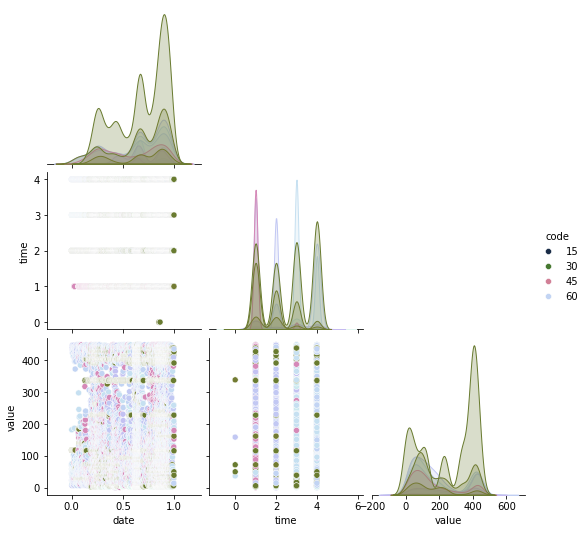
\includegraphics[width=0.8\textwidth]{1.png}
    \caption{\centering Vizuelizacija za korelaciju medu features-ima po verovatonosnoj distributivnoj
    funkciji (PDF) na target vrednost \texttt{code}}
\end{figure}

\section{Metodologija}
\subsection{Opis modela koji je dao najbolje rezultate}
%%%%%%%%%%%%%%
Meta-procenjivač (metod ansambla) nad više klasifikatora slučajnih stabala nad raznolikim poduzorcima skupa podataka koji se koriste pri ustanovljavanju proseka tačnosti predviđanja (prikaz na slici 7.) i upravljanje overfitting-om.\cite{ensamblerf}\cite{rf} Ističe se kao tehnika pomešati i kombinovati (preturb and combine; kreira više verzija datog grafa, primenjuje funkciju cena za čvorve pojedinačno za svaki graf, ukombinuje rezultate\cite{pnc}) namenjenog za stabla i sa time je uveden koncept nasumičnosti u konstrukcije klasifikacija. 

\begin{figure}[h!]
    \centering
    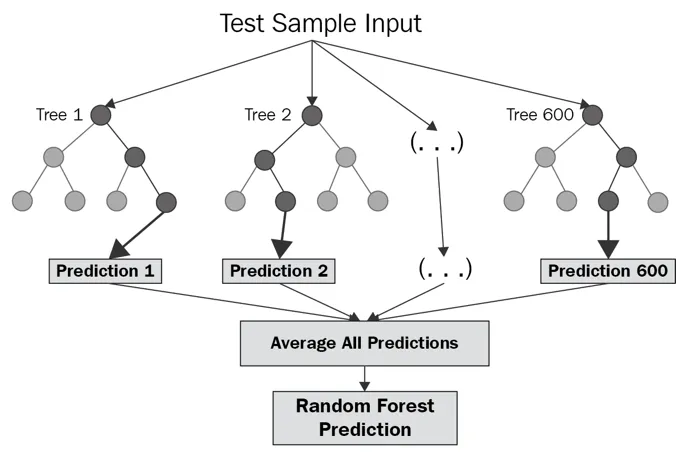
\includegraphics[width=0.5\textwidth]{image-6.png}
    \caption{Plan predviđanja slučajnih šuma.}
\end{figure}

Podržavaju proširenje na probleme više izlaza kao što je pomenuto u sekciji \hyperref[sec:mop]{2.2.1}.

Svako stablo u ansamblu građeno je iz uzorka sa zamenom (bootstrap uzorak) iz trening skupa.
Pri gradnji stabla podeli po svakom čvoru, najbolja podela je se pravi pri iscrpnoj pretrazi vrednosti features-a ili po nasumičnom skupu veličine naspram broja najviše mogućih features-a koja je unapred podešena. Cilj je izbeći visoku disperziju i overfitting procenjivača slučajnih šuma. Uvođenjem efekta nasumičnosti razložilo je greške pri predviđanju, a pri uzimanju proseka - neke greške su eliminisane. Zauzvrat, moguće je naići na blag porast cene u bias-u. 

Neki od kombinacije klasifikatora služe računanjem proseka, neki se koriste ``glasanjem'' za posebnu klasu.

\subsubsection{Unapred postavljeni parametri}
Glavni parametri zaslužni za prilagođavanje koji su korišćeni su \textit{broj procenjivača} i \textit{broj najviše features-a}, a može i da bude nekad \textit{broj stabala}. Preporuka je da budu veće vrednosti parametara, ističe se zahtevnost računa kao ishod. Nakon nekog kritičnog broja količine stabala ishoduje stagnaciji boljitka performansi. Sporedna veličina nasumičnih podskupova features-a se uzima u obzir kada se po čvoru vrši podela - što je niža to je veće umanjenje u disperziji, a veće pojačanje bias-a, sa manjom vrednošću je dosegnuta veća nasumičnost. Moguće je podesiti i \textit{najveću dubinu} i \textit{minimalan broj podela uzoraka}. Preporuka je da se izvrši cross-validation proces (ima moć da poredi i vrši odabir, manje se vezuje za određene koncepte nego druge tehnike predviđanja\cite{cv}) pri najbolje moguće podešenim parametrima. Moguće je podesiti zamenu uzorka (bootstrap mogućnost) gde greška generalizacije biva procenjena sa običnim uzorcima, uz bootstrap-bagging agregacije. 

Paralelizacija je moguća i ustanovljava paralelno izračunavanje predviđanja. Moguće je ekspilicitno podesiti broj zadataka koji će se izvršiti nad tom količinom jezgara u procesoru istovremeno. Vidljivo će biti uvećan performans pri radu sa većim brojem stabala ili pri radu sa većom količinom podataka na samom stablu.

Rangiranje srodnosti (npr. dubina) feature-a korišćeno je kada čvor odluke u stablu ustanovljava \textit{važnost feature-a} sve qdo predvidljivosti ciljane promenljive. Features-i korišćeni na vrhu stabla dprinose konačnom predviđanju krupnije frakcije ulaznih uzoraka. Očekivana frakcija uzoraka doprinosi pri proceni srodne važnosti features-a. U nekim sistemima frakcije uzoraka, kako feature doprinosi se uz kombinaciju umanjenja nečistosti po podeli pravi normalizovane procene za snagu predvđanja po feature-u. Po vršenju uprosečavanja procene moći predviđanja nad nekolicinom nasumičnih stabala se smanjuje disperzija takvih procena i njihovih korišćenja uz odabire feature-a - MDI (središnje opadanje u nečistosti).
Tim sračunavanjima feature važnosti zasnovanih na nečistosti sleduju 2 mane koje vode u zablude:
\begin{itemize}
    \item Sračunatim statistikama (funkcijom uzoraka; slučajnim promenljivama) svedenim iz trening skupa i sa time nas ne informiše o tome koji features-i su najvažniji da bi se napravile dobra predviđanja po priloženim skupovima podataka.
    \item Daje se prednost features-ima visokog kardinaliteta, pa i više jednoznačnih vrednosti. Permutacija važnosti feature-a (tehnika za obuku modela po statističkim performansama, korisna za nelinearne, neprovidne procenjivače koji uključuju nasumično pretumbavanje vrednosti posebnog feature-a i posmatranje degradacije rezultata ocene modela; ustanovljava se koliko se model osanja na određeni feature)\cite{permutation} je alternativa sračunavanjima feature važnosti zasnovanih na nečistosti, i eliminacija problema oslanjanja na feature, prikaz na slici 8. Dovodi se pojam \textit{važnosti permutacija} naspram MDI-a.
\end{itemize}
    \begin{figure}[h!]
        \centering
        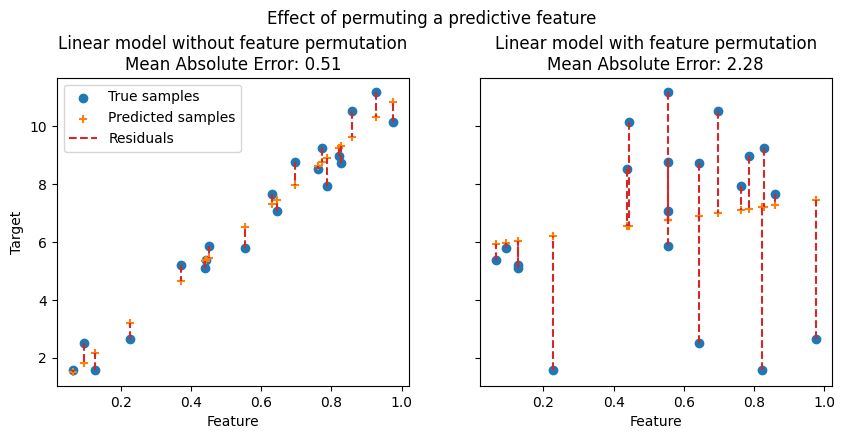
\includegraphics[width=0.5\textwidth]{image-9.png}
        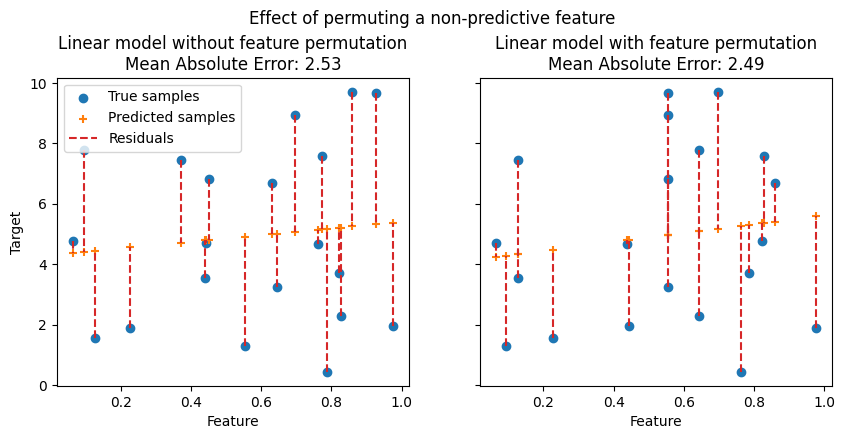
\includegraphics[width=0.5\textwidth]{image-7.png}
        \caption{Grafici sračunavanjima feature važnosti zasnovanih na nečistosti i permutacija važnosti feature-a (po kolonama) u okolnostima svojstva (ne)predvidljivog feature-a (po redovima).}
    \end{figure}
    
    Na slici 9. je dat primer korišćenja ekstremnih slučajnih šuma koji demonstriraju primenu feature važnosti po primeru individualnih piksela za svrhe prepoznavanje lica, što je svetlija tačka piksela to je važnost feature-a poklopljena pri funkcije procene predviđanja.
    \begin{figure}[h!]
        \centering
        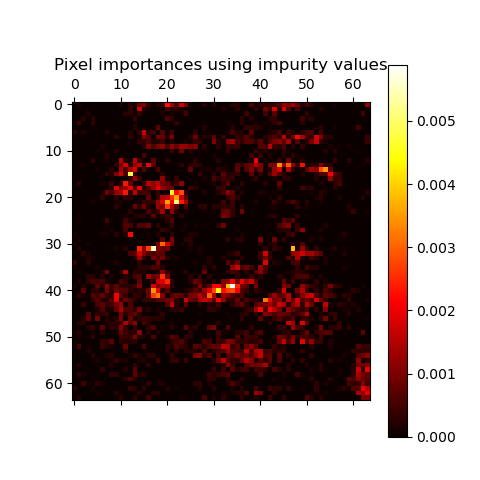
\includegraphics[width=0.32\textwidth]{image-8.png}
        \caption{Važnost piksela sa paralelnim slučajnim šumama, pri prepoznavanju lica.}
    \end{figure}

 

%%%%%%%%%%%%%%%
\newpage
Realizovana je klasifikacija \textbf{slučajnih šuma sa optimizacijom hiperparametara} 

\begin{verbatim}
    Best case:
RandomForestClassifier(max_depth=60, min_samples_leaf=2, min_samples_split=10,
                       n_estimators=16)
\end{verbatim}

korišćenjem \verb|RandomForestClassifier|\cite{RFC} i \verb|GridSearchCV|. U promenljivu \verb|param_grid| smešteni su parovi ključ, vrednost za koncepte:
\begin{itemize}
    \itemsep0em
    \item \verb|n_estimators = 16| - broj stabala odlučivanja u šumi, podrazumeva se da bude 100.
    \item \verb|max_depth = 60| - najveća dubina stabla odluke koja je uzeta u razmatranje.
    \item \verb|min_samples_leaf = 2| -  minimalan broj uzoraka u čvorovima listova u stablu, tačka podele ma koje dubine će biti uvažena ako se ustanovi toliki broj uzoraka trening skupa i sa leve i sa desne grane. Utiče na \textit{smooth}-ovanje. Zaokruživanje broja vrši na više.
    \item \verb|min_samples_split = 10| - minimalan potreban broj uzoraka da bi se desila podela, ako nije \verb*|int| tipa onda če da vrši zaokruživanje broja naviše.
    % \item \verb|bootstrap| - koriste se se bootstrap uzorci pri gradnji stabala, inače je korišćen čitav skup podataka za izgradnju stabala (što je podrazumevan slučaj1).
\end{itemize} 
\verb*|GridSearchCV| radi isprobavanje svakog ponaosob hiperparametra nad klasifikatorom i stratifikovan cross-validation postupak na 10 fold-ova. Izvlači se najbolji ishod evaluacija pri predviđanju test skupom nad obučenim modelom. 

\begin{lstlisting}[language=Python, caption={\centering Slučajne šume}]
print("====================================")
    from sklearn.model_selection import GridSearchCV
    from sklearn.ensemble import RandomForestClassifier

    print('Random Forest prediction:')
    RF = RandomForestClassifier()
    param_grid = {
        'n_estimators': np.arange(start=4, stop=20, step=4),
        'max_depth': list(range(10, 110, 50)) + [None],
        'min_samples_split': [2, 5, 10],
        'min_samples_leaf': [1, 2, 4],
        'bootstrap': [True, False]
    }
    RF_grid = GridSearchCV(estimator = RF,
                            param_grid=param_grid, verbose=0, 											cv=10, n_jobs=-1)
    RF_grid.fit(x_train,y_train)
    prediction=RF_grid.predict(x_test)
    print('Best case:')
    print(RF_grid.best_estimator_)
\end{lstlisting}

\subsection{Način na koji su rezultati predstavljeni}
U daljem tekstu biće obrađene diskusije oko rezultata obavljenih evaluacija nad modelima i sa (gde će biti ukazano na parametre koji su najboljeg mogućeg ishoda) i bez optimizacija hiperparametara. Proračun metrika po svakoj ciljanoj vrednosti vrši se sagledanjem vrednosti koje su ključne kao na slici 5. i 6. 
\begin{figure}[h]
    \centering
    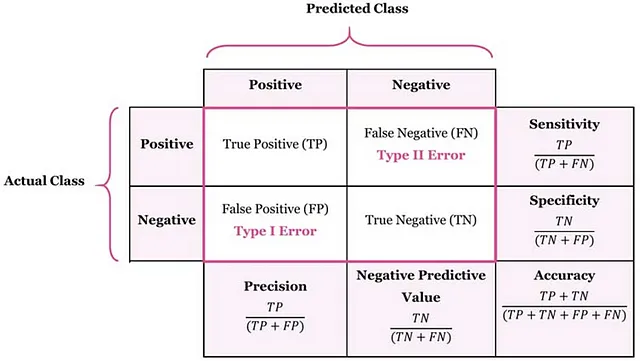
\includegraphics[width=0.8\textwidth]{2.png}
    \caption{\centering Izračuvanje bitnih metrika}
\end{figure}

\begin{figure}[h]
    \centering
    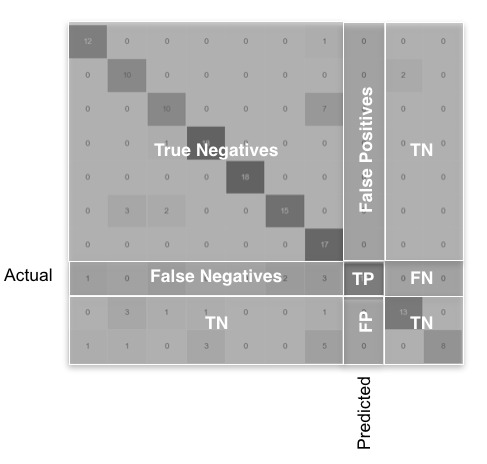
\includegraphics[width=0.35\textwidth]{3.png}
    \caption{\centering Konfuziona matrica multiklasnog skupa podataka}
\end{figure}
Senzitivitnosti (recall) ističe koliko validacijom model dobro predviđa u skladu 2 uparena skupa. Dok specifičnost ističe koliko se za 2 uparena skupa poklopljeno loše predviđa po modelu. Preciznost govori koliko je model sposoban da poklopi činjeničnu evaluaciju naspram nečinjenične sa obrascem skupa (test skupa) predvidjanog nad trening skupom. Tačnost u ovom slučaju govori koliko činjenični skup je pogodan naspram modela. F1-score računat po formuli $2*\frac{precision*recall}{precision+recall}$ koji je kombinacija senzitivnosti i preciznosti. Takođe se daju statističke vrednosti:
\begin{enumerate}
    \item koliki je krajnji accuracy,
    \item macro avg - metrike (preciznost, senzitivnost, f1) se izračunavaju prosekom podjednakog udela svake vrednosti ponaosob,\cite{metrics1}\cite{metrics2}
    \item weighted avg - metrike se računaju tako što na prosek utiče težinski udeo po zastupljenosti vrednosti klasifikatornog atributa ponaosob.
\end{enumerate}
Formiranje konfuzione matrice koja služi za prikaz zastupljenosti pri poklapanju skupa podataka nakon predikcija sa onim koji su dati pre predikcija, prikaz konfuzione matrice, zasebna izdvajanja metrika  za svaku klasu zasebno je obavljena.

\newpage

\section{Rezultati najboljeg modela koji je zapažen}
U implementaciji 11. konstruisan je izveštaj klasifikacije i konfuzione matrice nakon obuke nad trening skupom ulaznih i izlaznih vrednosti; predikcije nad test skupom ulaznih vrednosti. Izveštaj i matrica se grade ustanovljavanjem poklapanja predviđenog i stvarne target vrednosti za features-e koji su posmatrani (broj poklapanja po klasi u izlazu 1. je predstavljen kao \verb|support|, a na slici 7. je na dijagonali).
\begin{lstlisting}[language=Python, caption={\centering Implementacija generisanja izveštaja i matrice klasifikacije}]
from sklearn.metrics import classification_report
from sklearn.metrics import confusion_matrix
...
report = classification_report(list(y_test), prediction)
print(report)
    
cm=confusionMatrix(list(y_test),prediction, "Random Forst w/ optimization")
\end{lstlisting}

Najzastupljenija target vrednost \verb|code| je 33, tj. regularno insulinsko ubrizgivanje sa 1785 instanci, a i najprecizniji sa 84\%, i senzitivnosti od 91\%, f1-score-om od 87\%.

Tačnost je 71\%, od ukupno 5478 instanci. Mikro-prosečnost za preciznost daje 40\%, senzitivnost 36\%, a f1-score 36\%. Težinska-prosečnost za preciznost gradi 69\%, senzitivnost 71\%, f1-score 70\%.
\renewcommand\lstlistingname{Izlaz}
\renewcommand\lstlistlistingname{Izlaz}
\setcounter{lstlisting}{0}
\begin{lstlisting}[caption={\centering Izveštaj o klasifikaciji o ovom modelu}]
              precision    recall  f1-score   support
          33       0.84      0.91      0.87      1785
          34       0.78      0.76      0.77       703
          35       0.74      0.70      0.72       197
          48       0.60      0.58      0.59       399
          56       0.40      0.10      0.16        20
          57       0.36      0.12      0.18       174
          58       0.62      0.69      0.65       677
          59       0.00      0.00      0.00         2
          60       0.71      0.73      0.72       541
          61       0.00      0.00      0.00        14
          62       0.64      0.72      0.68       571
          63       0.50      0.09      0.15        35
          64       0.31      0.12      0.18       153
          65       0.32      0.36      0.34        56
          66       0.62      0.70      0.66        33
          67       0.34      0.48      0.40        46
          68       0.00      0.00      0.00         6
          69       0.08      0.08      0.08        13
          70       0.26      0.24      0.25        21
          71       0.14      0.06      0.08        17
          72       0.12      0.07      0.09        15

    accuracy                           0.71      5478
   macro avg       0.40      0.36      0.36      5478
weighted avg       0.69      0.71      0.70      5478
\end{lstlisting}
\begin{figure}[h]
    \centering
    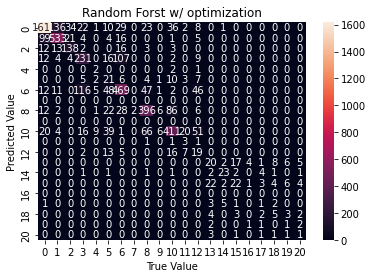
\includegraphics[width=1\textwidth]{4.png}
    \caption{\centering Konfuziona matrica multiklasnog skupa podataka za ovaj model algoritma}
\end{figure}
\newpage
\section{Zakljućak}
Predstavljeni slučajevi tačnosti za svaki model klasifikacije na tabeli 1. može se uočiti da je najbolji model slučajnih šuma sa optimizacijom hiperparametara. 

Može se uočiti da optimizacija hiperparametara većinski nije neophodna gledajući rezultate sveukupno.

\begin{table}[h]
    \centering
    \begin{tabular}{|r|c|c|}
    \hline
    \textbf{Klasifikator} & \textbf{Tačnost sa GridSearchCV} & \textbf{Tačnost bez GCV} \\
    \hline
    Stablo odlučivanja & 60\% & 67\% \\
    \hline
    Slučajne šume & 71\% & 69\% \\ 
    \hline
    KNN & 70\% & 70\% \\ 
    \hline
    \end{tabular}
    \caption{Prikaz tačnosti klasifikatora sa i bez primene optimizacije hiperparametara.} 
\end{table}

Najbolji model je imao rezultate bolje od drugih, jer je tačan i moćan model, rukuje overfitting-om efikasno, rukuje feature-om naspram važnosti, kombinuje više stabala (zbog toga je pouzdaniji od stabala odlučivanja), radi efikasno sa međusobno nelinearnim features-ima. 

Stablo odlučivanja nije pogodno za rad sa outliers-ima, nije pogodno u slučaju pristasnosti, kontinualne vrednosti (kao skalirani enkodirani datum ovde), zarobi se u lokalnom optimalnom rezultatu.

Iako se približno jednako pokazao KNN algoritam (u oba slučaja) sa slučajnim šumama sa optimizacijom hiperparametara. Ovde je, ipak, veći broj uzoraka bio zastupljen i to je bio ograničavajući faktor. Takođe je loše raditi sa šumovima i redudantnim vrednostima features-a.
\newpage

%%%%%%%%%%%%%%%%%%%%%%%%%%%%%%%%%%%%%%%%%%%%%%%%%%%%%%%%%%%%%%%%%
% \begin{lstlisting}[language=Python, caption=Predprocesiranje podataka i navođenje modula koji će se koristiti] 
%     print()
%     
    
%     from sklearn.model_selection import GridSearchCV
%     from sklearn.linear_model import LogisticRegression
%     from sklearn.tree import DecisionTreeClassifier
%     from sklearn.ensemble import RandomForestClassifier
%     from sklearn.naive_bayes import GaussianNB
%     from sklearn.naive_bayes import MultinomialNB
%     from sklearn.naive_bayes import BernoulliNB
%     from sklearn.naive_bayes import CategoricalNB
%     from sklearn.naive_bayes import ComplementNB
%     from sklearn.svm import SVC
%     from sklearn.neighbors import KNeighborsClassifier
    
%     def confusionMatrix(y_true,y_pred,title):
%         cm=confusion_matrix(y_pred,y_true)
%         plt.figure()
%         sb.heatmap(cm, annot=True, fmt='0')
%         plt.title(title)
%         plt.xlabel('True Value')
%         plt.ylabel('Predicted Value')
    
    
    
    
%     print("====================================")
%     print('Decision Tree prediction:')
%     DT = DecisionTreeClassifier()
%     param_grid = {
%         'criterion': ['gini', 'entropy'],
%         'max_depth': np.arange(3, 15, step=6),
%         'min_samples_leaf': np.arange(1, 10, step=3),
%         'ccp_alpha': [0, 0.1, 0.2]
%     }
%     DT_grid = GridSearchCV(estimator = DT,
%                            param_grid=param_grid, verbose=0, 									   cv=10, n_jobs=-1)
%     DT_grid.fit(x_train,y_train)
%     prediction=DT_grid.predict(x_test)
%     print('Best case:')
%     print(DT_grid.best_estimator_)
%     print()
%     report = classification_report(list(y_test), prediction)
%     print(report)
    
%     cm=confusionMatrix(list(y_test),prediction, "Decision Tree w/ optimization")
    
    
%     print("------------------------------------")
%     print(f'Decision Tree prediction without optimization:')
%     DT.fit(x_train,y_train)
%     prediction=DT.predict(x_test)
    
%     print()
%     report = classification_report(list(y_test), prediction)
%     print(report)
    
%     cm=confusionMatrix(list(y_test),prediction, "Random Forst ")
    
%     print("====================================")
%     print('Random Forest prediction:')
%     RF = RandomForestClassifier()
%     param_grid = {
%         'n_estimators': np.arange(start=4, stop=20, step=4),
%         'max_depth': list(range(10, 110, 50)) + [None],
%         'min_samples_split': [2, 5, 10],
%         'min_samples_leaf': [1, 2, 4],
%         'bootstrap': [True, False]
%     }
%     RF_grid = GridSearchCV(estimator = RF,
%                             param_grid=param_grid, verbose=0, 											cv=10, n_jobs=-1)
%     RF_grid.fit(x_train,y_train)
%     prediction=RF_grid.predict(x_test)
%     print('Best case:')
%     print(RF_grid.best_estimator_)
%     print()
%     report = classification_report(list(y_test), prediction)
%     print(report)
    
%     cm=confusionMatrix(list(y_test),prediction, "Random Forst w/ optimization")
    
%     print("------------------------------------")
%     print(f'Random Forest prediction without optimization:')
%     RF.fit(x_train,y_train)
%     prediction=RF.predict(x_test)
%     report = classification_report(list(y_test), prediction)
%     print(report)
    
%     cm=confusionMatrix(list(y_test),prediction, "Random Forst ")
    
%     print("====================================")
%     print(f'KNN prediction:')
%     estimator_KNN = KNeighborsClassifier(algorithm='auto')
%     parameters_KNN = {
%         'n_neighbors': (1,10),
%         'leaf_size': (20,40),
%         'p': (1,2),
%         'weights': ('uniform', 'distance'),
%         'metric': ('minkowski', 'chebyshev')	   
%     } 
%     # with GridSearch
%     grid_search_KNN = GridSearchCV(
%         estimator=estimator_KNN,
%         param_grid=parameters_KNN,
%         scoring = 'accuracy',
%         n_jobs = -1,
%         cv = 5
%     )
%     grid_search_KNN.fit(x_train,y_train)
%     prediction=grid_search_KNN.predict(x_test)
%     print('Best case:')
%     print(grid_search_KNN.best_estimator_)
%     print()
%     report = classification_report(list(y_test), prediction)
%     print(report)
%     cm=confusionMatrix(list(y_test),prediction, "KNN w/ optimization")
    
%     print("------------------------------------")
%     print(f'KNN prediction without optimization:')
%     estimator_KNN = KNeighborsClassifier(algorithm='auto')
%     estimator_KNN.fit(x_train,y_train)
%     prediction=estimator_KNN.predict(x_test)
%     report = classification_report(list(y_test), prediction)
%     print(report)
    
%     cm=confusionMatrix(list(y_test),prediction, "Random Forst ")
% \end{lstlisting}

\newpage

\begin{thebibliography}{1}
    \bibitem{diabetes}
    Diabetes - UCI Machine Learning Repository,

    \url{https://archive.ics.uci.edu/dataset/34/diabetes},

    Datum pristupa: \today,
    \bibitem{pd}
    pandas.read\_csv,

    \url{https://pandas.pydata.org/pandas-docs/stable/reference/api/pandas.read_csv.html}, Datum pristupa: \today,

    \bibitem{sb}
    seaborn.pairplot,

    \url{https://seaborn.pydata.org/generated/seaborn.pairplot.html},

    Datum pristupa: \today,
    \bibitem{plt}
    matplotlib.pyplot.figure,

    \url{https://matplotlib.org/stable/api/_as_gen/matplotlib.pyplot.figure.html},

    Datum pristupa: \today,
    \bibitem{np}
    numpy.reshape,

    \url{https://numpy.org/doc/stable/reference/generated/numpy.reshape.html},

    Datum pristupa: \today,
    \bibitem{le}
    LabelEncoder,

    \url{https://scikit-learn.org/stable/modules/generated/sklearn.preprocessing.LabelEncoder.html},

    Datum pristupa: \today,
    \bibitem{ms}
    MinMaxScaler,

    \url{https://scikit-learn.org/dev/modules/generated/sklearn.preprocessing.MinMaxScaler.html},

    Datum pristupa: \today,
    \bibitem{tts}
    train\_test\_split,

    \url{https://scikit-learn.org/stable/modules/generated/sklearn.model_selection.train_test_split.html},

    Datum pristupa: \today,
    \bibitem{RFC}
    RandomForestClassifier,

    \url{https://scikit-learn.org/stable/modules/generated/sklearn.ensemble.RandomForestClassifier.html},

    Datum pristupa: \today,

    \bibitem{gscv}
    GridSearchCV,

    \url{https://scikit-learn.org/stable/modules/generated/sklearn.model_selection.GridSearchCV.html},

    Datum pristupa: \today,
    \bibitem{ensamblerf}
    1.11.2. Random forests and other randomized tree ensembles, 
    
    \url{https://scikit-learn.org/stable/modules/ensemble.html#forest}, 
    
    Datum poslednjeg pristupa: \today
    \bibitem{rf}
    sklearn.ensemble.RandomForestClassifier, 
    
    \url{https://scikit-learn.org/stable/modules/generated/sklearn.ensemble.RandomForestClassifier.html}, 
    
    Datum poslednjeg pristupa: \today
    \bibitem{pnc}
    Tixier A.J.P., 2018., Perturb and Combine to Identify Influential
Spreaders in Real-World Networks, 

    \url{https://arxiv.org/pdf/1807.09586.pdf}, 
    
    Datum poslednjeg pristupa: \today
   \bibitem{cv}
   Brownlee J., 2023. A Gentle Introduction to k-fold Cross-Validation, 
   
   \url{https://machinelearningmastery.com/k-fold-cross-validation/}, 
   
   Datum poslednjeg pristupa: \today
   \bibitem{permutation}
   4.2. Permutation feature importance, 
   
   \url{https://scikit-learn.org/stable/modules/permutation_importance.html#permutation-importance}, 
   
   Datum poslednjeg pristupa: \today

   \bibitem{metrics1}
    Machine Learning Model Evaluation Metrics part 2: Multi-class classification, 
    
    \url{https://www.mariakhalusova.com/posts/2019-04-17-ml-model-evaluation-metrics-p2/}, 
    
    Datum poslednjeg pristupa: \today
    \bibitem{metrics2}
    Classification metrics: Multiclass and multilabel classification, 
    
    \url{https://scikit-learn.org/stable/modules/model_evaluation.html#multiclass-and-multilabel-classification}, 
    
    Datum poslednjeg pristupa: \today
\end{thebibliography}
\end{document}
